\begin{ZhChapter}
    \chapter{Related Work}
    In the following sections, we will introduce the concept of metaheuristics \cite{yang2010nature,yang2011metaheuristic} . Then, we will discuss the importance of loss functions and their role in deep learning \cite{deepLearning} models. Finally, we will explore image classification \cite{rawat2017deep} and its real-life applications.

    \section{Metaheuristic}
    In the following section, we will discuss metaheuristic and some of the most famous metaheuristic algorithms include Evolving Algorithm (EA), Genetic Algorithm (GA), and Genetic Programming (GP). After that, we will introduce related research in the GP domain.
    \subsection{Overview of Metaheuristic}
    Metaheuristic \cite{glover1986future} was first proposed by \citeauthor{glover1986future}. It can be regarded as a high-level procedure used to find solutions to optimization problems or other issues that conventional algorithms cannot solve. Within metaheuristics, an important concept is that these procedures must find a potentially optimal solution under reasonable computational costs or insufficient information. In this paper, we will primarily focus on nature-inspired metaheuristics \cite{yang2010nature}. In these methods, a common approach is to use a population-based strategy to find the optimal solution. Within a population, each individual typically represents a potential solution. We perform various operations on the individuals within the population to achieve our goal of approximating the optimal solution. A subset of specialized algorithms falls under population-based methods \cite{enwiki:1255593755}, commonly referred to as evolving algorithms (EAs) \cite{muhlenbein1988evolution}. Commonly used methods within EAs include genetic algorithms (GA) \cite{kumar2010genetic}, genetic programming (GP) \cite{geneticProgramming} , evolutionary programming (EP) \cite{yao1999evolutionary}, and differential evolution (DE) \cite{das2010differential}. The relationship between Metaheuristic, EA, GA, GP, EP and DE is illustrated in the figure \ref{fig: relationshipMap}. We will briefly discuss EAs and GAs, and then we will focus primarily on GPs in the following paragraph.
    \begin{figure*}[htbp]
        \centering
        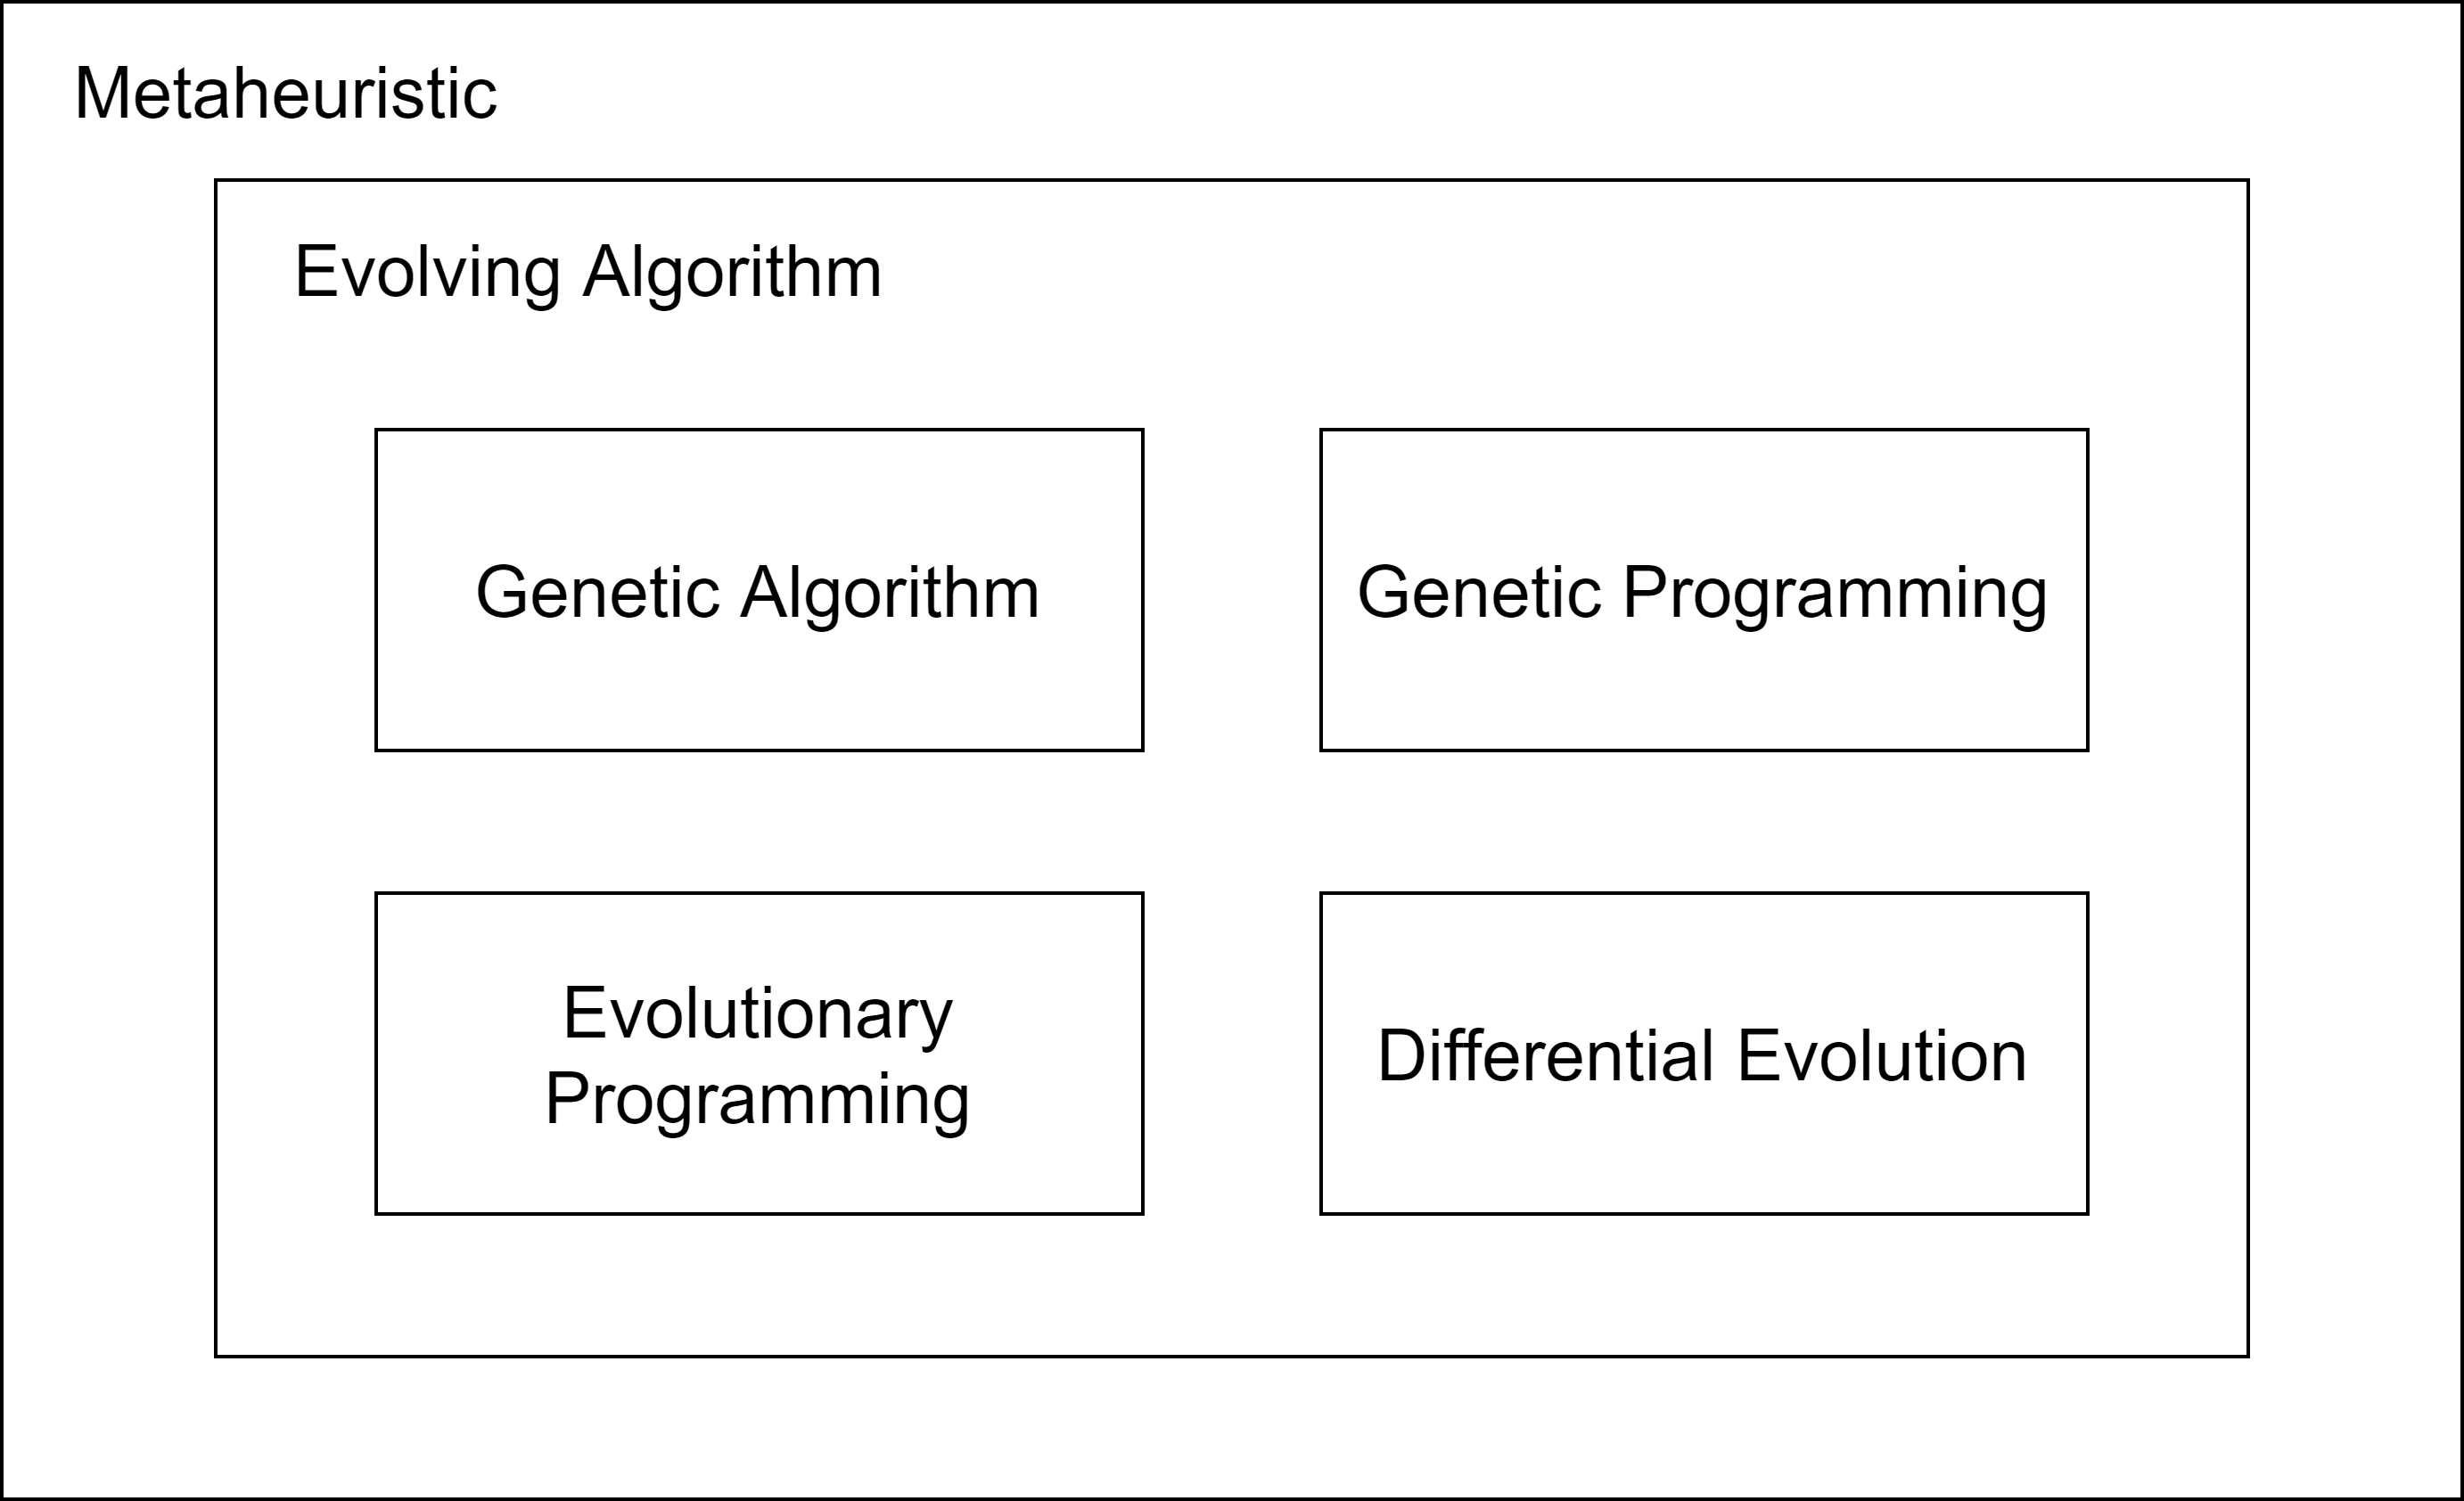
\includegraphics[width = 0.75\textwidth]{image/metaheuristic.png}
        \caption{Relationship between metaheuristic, EA, GA, GP, EP, and DE}
        \label{fig: relationshipMap}
    \end{figure*}
    \subsection{Evolving Algorithms}
    EAs can be described as algorithms inspired by the concept of "survival of the fittest \cite{paul1988selection}." These algorithms often take cues from natural evolutionary mechanisms to create algorithms that mimic animal behavior in the search for optimal solutions. Common examples include Ant Colony Optimization (ACO) \cite{dorigo2006ant}, GA, and Particle Swarm Optimization (PSO) \cite{kennedy1995particle}. The common EA procedure is shown in figure \ref{fig: EA}. In this type of algorithm, the typical approach is to initialize a population, which consists of several individuals. Each individual represents a potential optimal solution. After initializing the population, we usually set a number to represent how many generations we want this population to evolve. Before the start of each generation, a special function is used to calculate the fitness value of each individual, determining their level of excellence. Next, we perform selection, mutation, and crossover on the population. Selection involves choosing individuals based on their fitness to reproduce the next generation. Mutation generally refers to making random changes to an individual, while crossover combines the characteristics of two individuals to create the next generation. These steps are repeated until the predefined number of generations is reached, or the individuals fail to achieve the expected results, leading to a forced stop. Ultimately, the best individual in the population is obtained as the solution.
    \begin{figure*}[htbp]
        \centering
        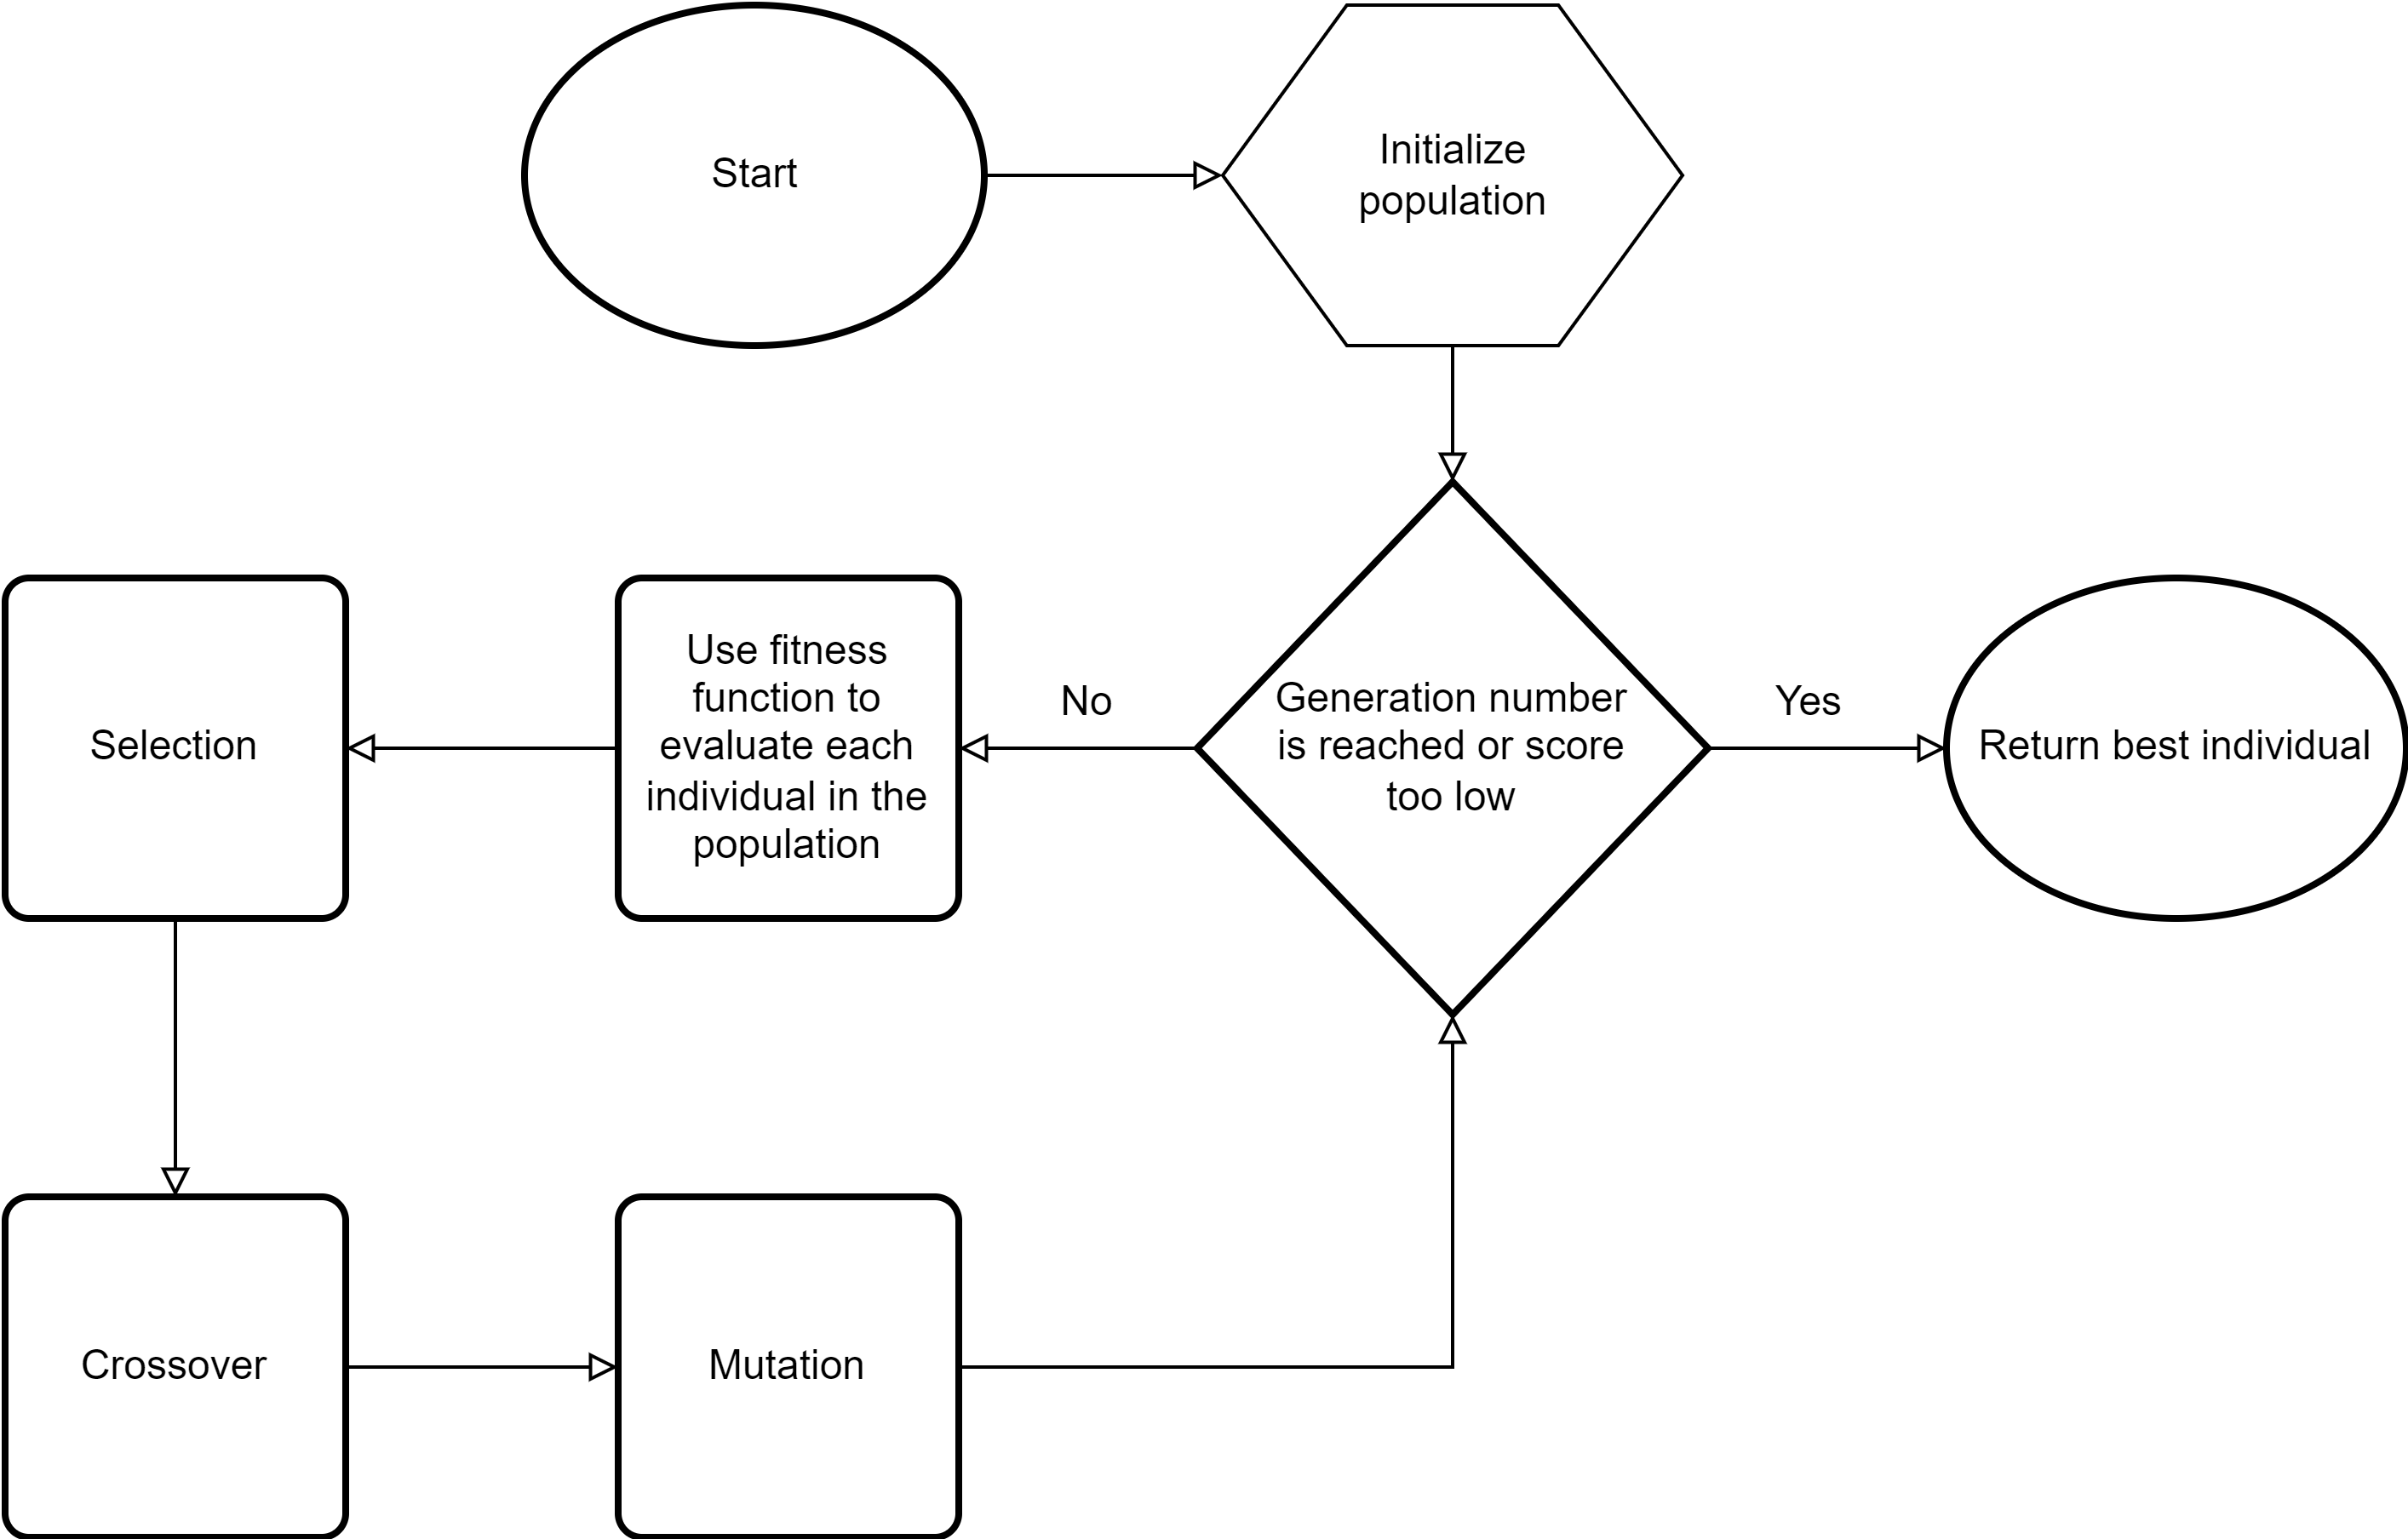
\includegraphics[width = 0.75\textwidth]{image/EA.png}
        \caption{Flowchart for EA}
        \label{fig: EA}
    \end{figure*}
    \subsection{Genetic Algorithms \& Genetic Programming}
    GA is considered a type of EA, utilizing the representation of each solution in the form of chromosomes to perform selection, mutation, and crossover. GP is regarded as a special case of GAs, but due to its versatility and practicality, it is seen as a reliable solution. Unlike GAs, GP typically uses a more robust encoding method to represent chromosomes. For instance, GAs often use strings to represent chromosomes, which can present potential issues that need to be addressed, such as the priority of operations for each symbol or the validity of the equation itself. As shown in the figure \ref{fig: GPandGA}, if we want to express the function $(x + y) ÷ (5 * x)$ in GA, the chromosome representation of this function will be $x + y\ ÷\ 5 * x$. Without the proper parentheses, it can easily cause confusion. In contrast, GP usually represents chromosomes as trees, a method that can employ predefined traversal techniques to avoid these issues. As illustrated in the figure \ref{fig: GPandGA}, the same function represented by GA can be expressed through a tree structure in GP. By specifying the use of inorder traversal, we can obtain the same function. It is worth noting that in GAs and GP, we can leverage their inherent ability to evolve automatically to find a reasonable optimal solution without having an in-depth understanding of the knowledge domain related to the problem we aim to solve. In the following paragraphs, we will introduce related research.

    \begin{figure*}[htbp]
        \centering
        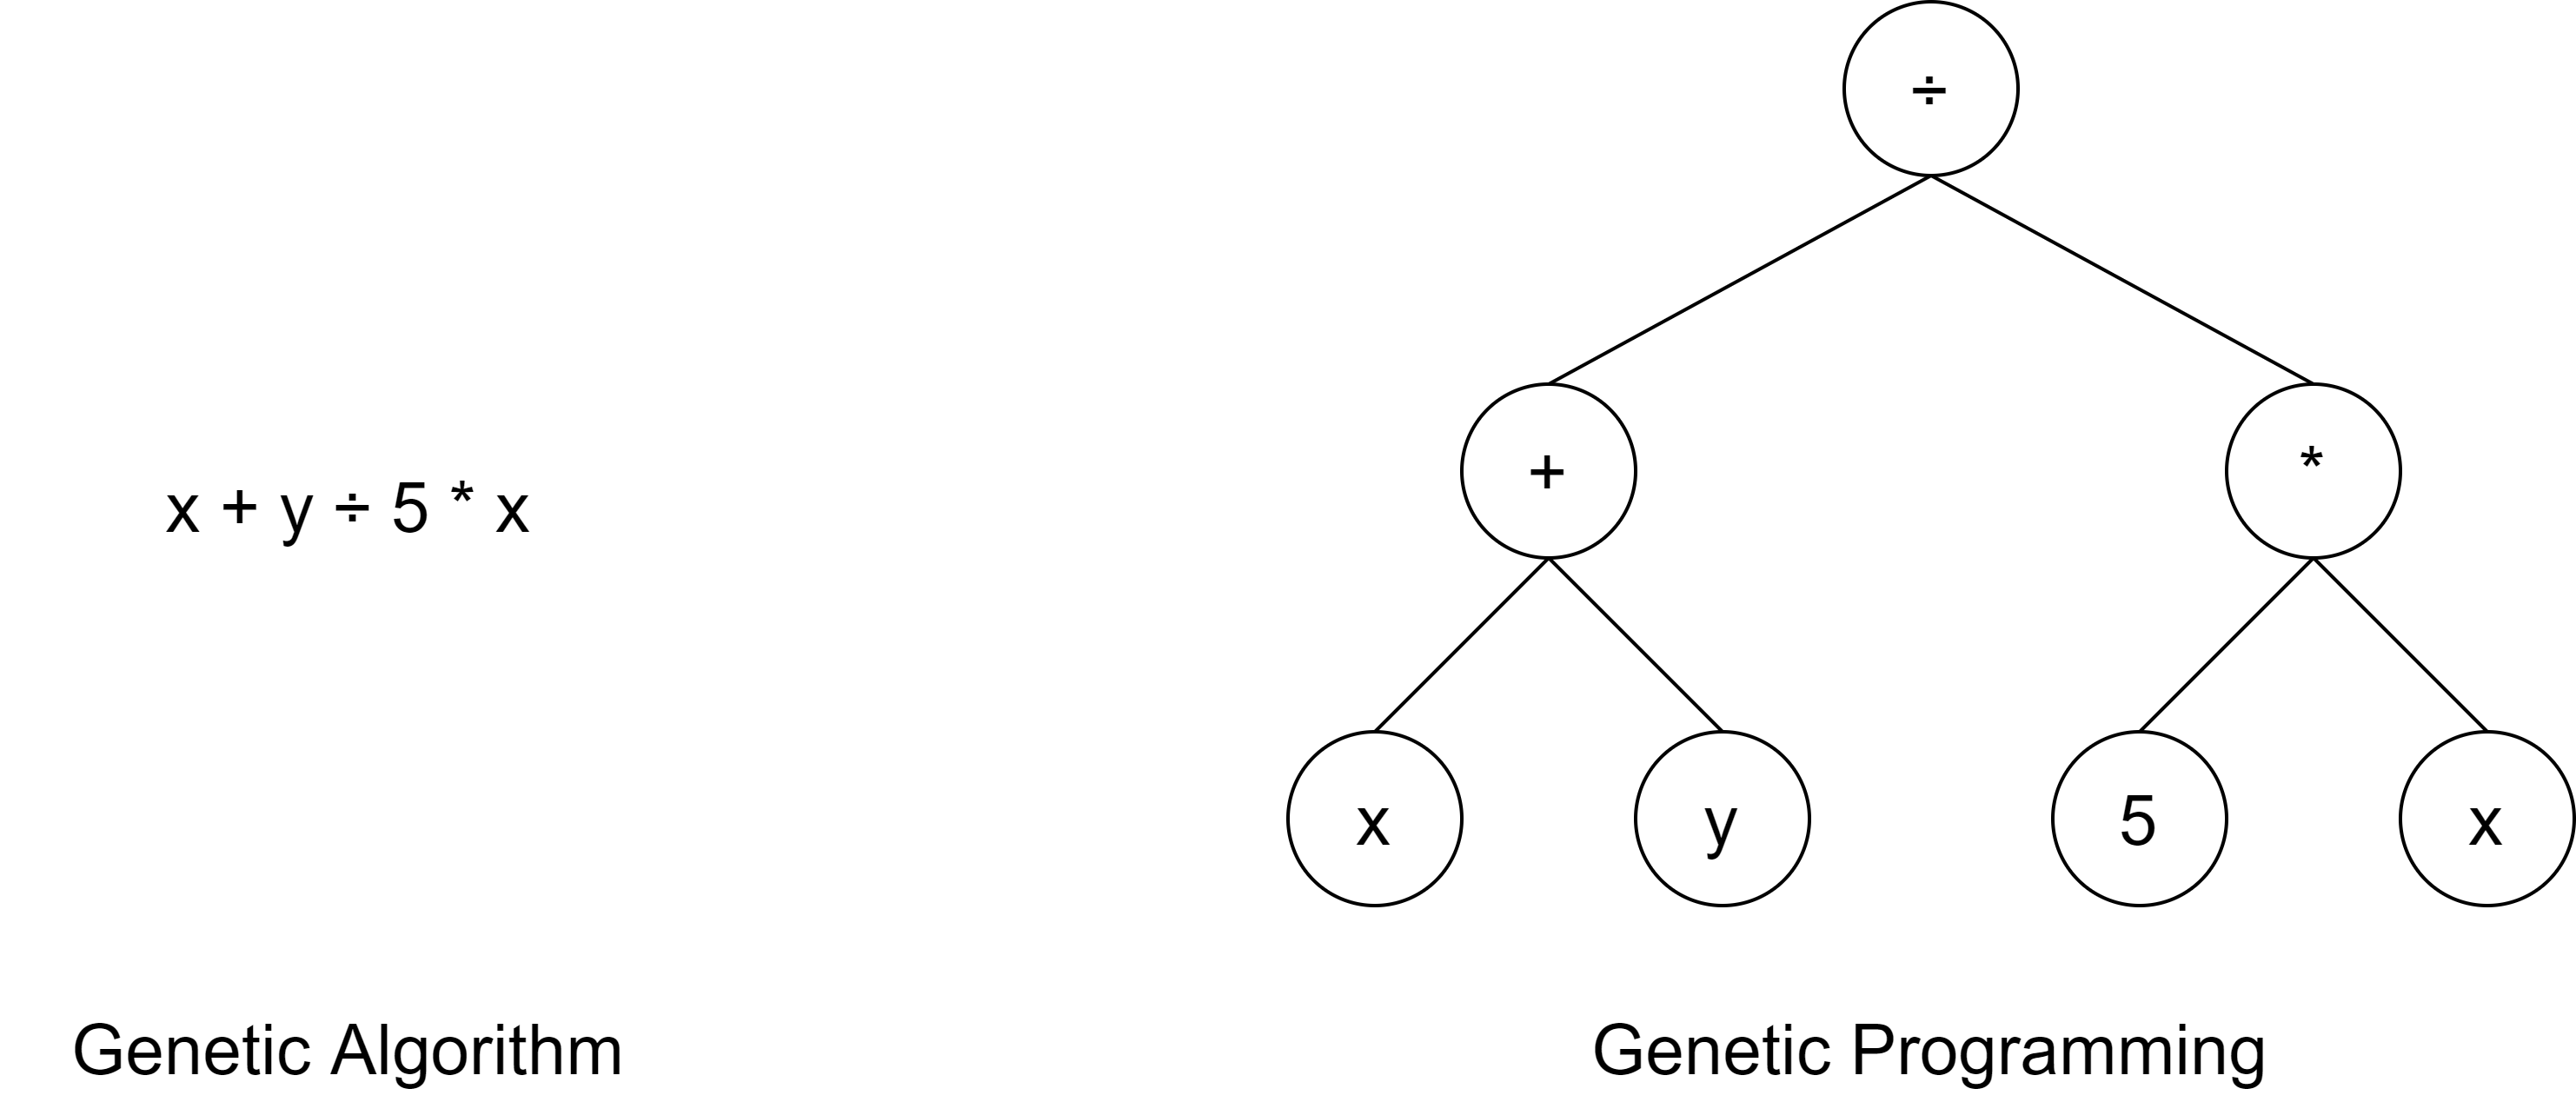
\includegraphics[width = 0.75\textwidth]{image/GPandGA.png}
        \caption{Different chromosome representation between GA and GP}
        \label{fig: GPandGA}
    \end{figure*}

    In \cite{coreyes2022evolvingreinforcementlearningalgorithms}, \citeauthor{coreyes2022evolvingreinforcementlearningalgorithms} proposed a meta-learning reinforcement learning algorithm. They used computational graphs to represent algorithms. By doing so, algorithms could be identified, calculated, and optimized through Reinforcement Learning (RL) \cite{kaelbling1996reinforcement}. Notably, in this study, algorithms were represented as directed acyclic graphs (DAG) \cite{thost2021directedacyclicgraphneural} of nodes. Within the DAG , all nodes were classified into three categories: input nodes, parameter nodes, and operation nodes. Once the algorithms were represented as DAGs, they could be placed into RL for training and evaluation. In this proposed algorithm, they employed the concept of regularized evolution \cite{real2019regularized} to evolve a population formed by several randomized and known algorithms. The method was as follows: initialize the population with algorithms, evaluate each algorithm in the population and record their performance, then in a loop, repeatedly use a sample tournament \cite{goldberg1991comparative} to select algorithms, perform mutations on the algorithms by the mutator they designed, and evaluate them again until the loop ends. During the evaluation process, they trained and assessed the algorithms using RL, continuously testing the performance of each algorithm in different training environments. They also utilized normalized training performance to avoid numerical biases caused by varying environments. Through this approach, the study successfully created two algorithms, named DQNClipped and DQNReg, which outperformed classical control tasks.

    In \cite{akhmedova2024generationlossfunctionimage}, \citeauthor{akhmedova2024generationlossfunctionimage} proposed a genetic programming-based method to find a better function for the image classification training task. They encoded the loss functions into trees, with each tree considered an individual. All individuals were aggregated into a population. In this study, the population was evolved across multiple generations. Before the start of each generation, all individuals were evaluated. Each individual had a probability of undergoing crossover with an individual from a special external archive to create a new individual; otherwise, it would perform the crossover with another individual. Following this, two probabilistic decisions were made. If successful, the new individual could perform subtree mutation or one-point mutation, respectively. At the end of each generation, the fitness value of all individuals was re-evaluated. A certain number of low-scoring individuals were eliminated to the special external archive mentioned earlier, maintaining the stability of the population's size. After these steps, a new generation began, continuing until a predefined number of generations was reached.  By employing this method, this study successfully evolved an outstanding individual within the population, creating a function that could train an image classification model more effectively compared to Cross Entropy (CE) \cite{zhang2018generalized}.

    \section{Loss Function}
    In this section, we will first introduce deep learning model and explain how does it work. Secondly, we will discuss the importance of loss function and present some related researches.
    \subsection{Deep Learning Model}
    In recent years, due to the significant increase in the computational speed of GPUs, training deep learning models to solve a wide variety of problems has become widely regarded as a feasible and popular solution. The process of training a deep learning model is often divided into several steps: collecting the data needed to train the model, and adding ground truth values to the data according to the model's requirements. Ground truth can be thought of as the ideal answers we hope to achieve after the model's computation. Once the data collection is complete, these data sets are collectively referred to as the dataset. Typically, the dataset is divided into training sets, validation sets, and testing sets. Data from the training set are used to train the model, the validation set is used to evaluate the model's effectiveness after each training loop, and the testing set is used to calculate the model's final score and determine whether the model successfully achieves its designed purpose. It is worth noting that the testing set data should not be seen during training and validation phases. After dividing the dataset, we decide on the model's architecture. Common architectures include Fully Connected Networks (FCN) \cite{iliadis2018deep} and Convolutional Neural Networks (CNN) \cite{wu2017introduction}, etc. Then the training process can begin. During training, we compare the model's output with the ground truth of the training data and use a loss function to calculate the difference between the output and the ground truth. This guides the adjustment of the model's parameters. Therefore, the loss function significantly determines the effectiveness of model training, and this aspect will be explained further later. After adjusting the model, the next round of training begins, continuing until the training is deemed ineffective or a predetermined maximum number of iterations is reached.
    \subsection{Loss Function In Deep Learning Model}
    In section 2.2.1, we discussed the role of loss functions in deep learning models. Here, we would like to introduce some commonly used loss functions along with their advantages and disadvantages. Mean-Square Error (MSE) \cite{wang2009mean} is a loss function used for solving regression problems. It calculates the difference between the actual and predicted values, squares them, and then takes the average of these squared differences to obtain the final loss value. However, a notable disadvantage of MSE is that it amplifies the impact of outliers exponentially. Cross-Entropy (CE), unlike MSE, leverages probability concepts to help compute the error in classification tasks. In other words, CE measures the difference between the predicted probability and the true probability to calculate the error. CE can also be adapted to different types of classification tasks to better suit their requirements, with common variants including Binary CE Loss \cite{ruby2020binary} and Multiclass CE Loss \cite{plaquet2023powerset}.

    From the above paragraphs, it seems that using a single type of loss function to train all models is considered impractical. Therefore, researchers design different loss functions based on specific needs to calculate more appropriate loss values for the model. As the introduction above indicates, designing a loss function requires an in-depth understanding of the model and a clear grasp of how to define and calculate the loss value. Consequently, designing a loss function, similar to adjusting hyperparameters or model architecture, is considered as a challenging task that needs a deep understanding of the domain for effective design and adjustment.

    In \cite{gonzalez2020improvedtrainingspeedaccuracy}, \citeauthor{gonzalez2020improvedtrainingspeedaccuracy} proposed a meta-learning approach to create a loss function called Genetic Loss-function Optimization (GLO). Through their research, the authors experimentally found a loss function named de novo, created by GLO, outperforms the well-known CE loss in standard image classification tasks. Additionally, because GLO enables training to be completed in fewer steps, this method also enhances the speed and efficiency of the training process.

    In \cite{akhmedova2024generationlossfunctionimage}, \citeauthor{akhmedova2024generationlossfunctionimage} utilize GP to create a loss function that outperforms CE in image classification. The method described in the paper led to the creation of a loss function named Next Generation Loss (NGL). When trained with the Inception model, NGL outperforms CE on datasets such as CIFAR-10 \cite{CIFAR-10}, CIFAR-100 \cite{CIFAR-100}, and Fashion-MNIST \cite{xiao2017fashionmnistnovelimagedataset}. Additionally, it demonstrates excellent performance on larger datasets like  \cite{imagenet15russakovsky}. Furthermore, NGL is also effective in improving model performance in segmentation downstream tasks.

    From the above paragraphs, we can observe that numerous studies indicate that in image classification tasks, if a well-designed loss function is developed, it has the potential to outperform the most famous and widely regarded as the most effective CE loss function. However, as mentioned earlier, designing a loss function is usually considered a resource-intensive task. Therefore, the two studies discussed above have begun to use genetic programming to enable computers to automatically design a loss function that can effectively collaborate with a model in a specific domain and significantly improve the model's performance.

    \section{Image Classification}
    Image classification is a technique in computer vision that enables computers to identify what object present in an image. This technology is often used with image localization \cite{sattler2011fast}. Image localization determines the location of objects within an image, using bounding box \cite{he2019boundingboxregressionuncertainty} to enclose the areas where the objects are found. Additionally, object detection \cite{zhao2019object} is a similar technique to image classification and image localization. Unlike image classification and image localization, which focus on identifying one label per image, object detection can identify multiple labels in a single image. The difference between image classification, image localization and object detection is illustrated in the figure \ref{fig: IC&OD}. We can see that image classification is capable of recognizing which label the entire image belongs to, whereas image localization identifies which specific regions of the image belong to which labels. Object detection is a more complex  technique, which can identify multiple labels and also mark the object by using bounding boxes.
    \begin{figure*}[htbp]
        \centering
        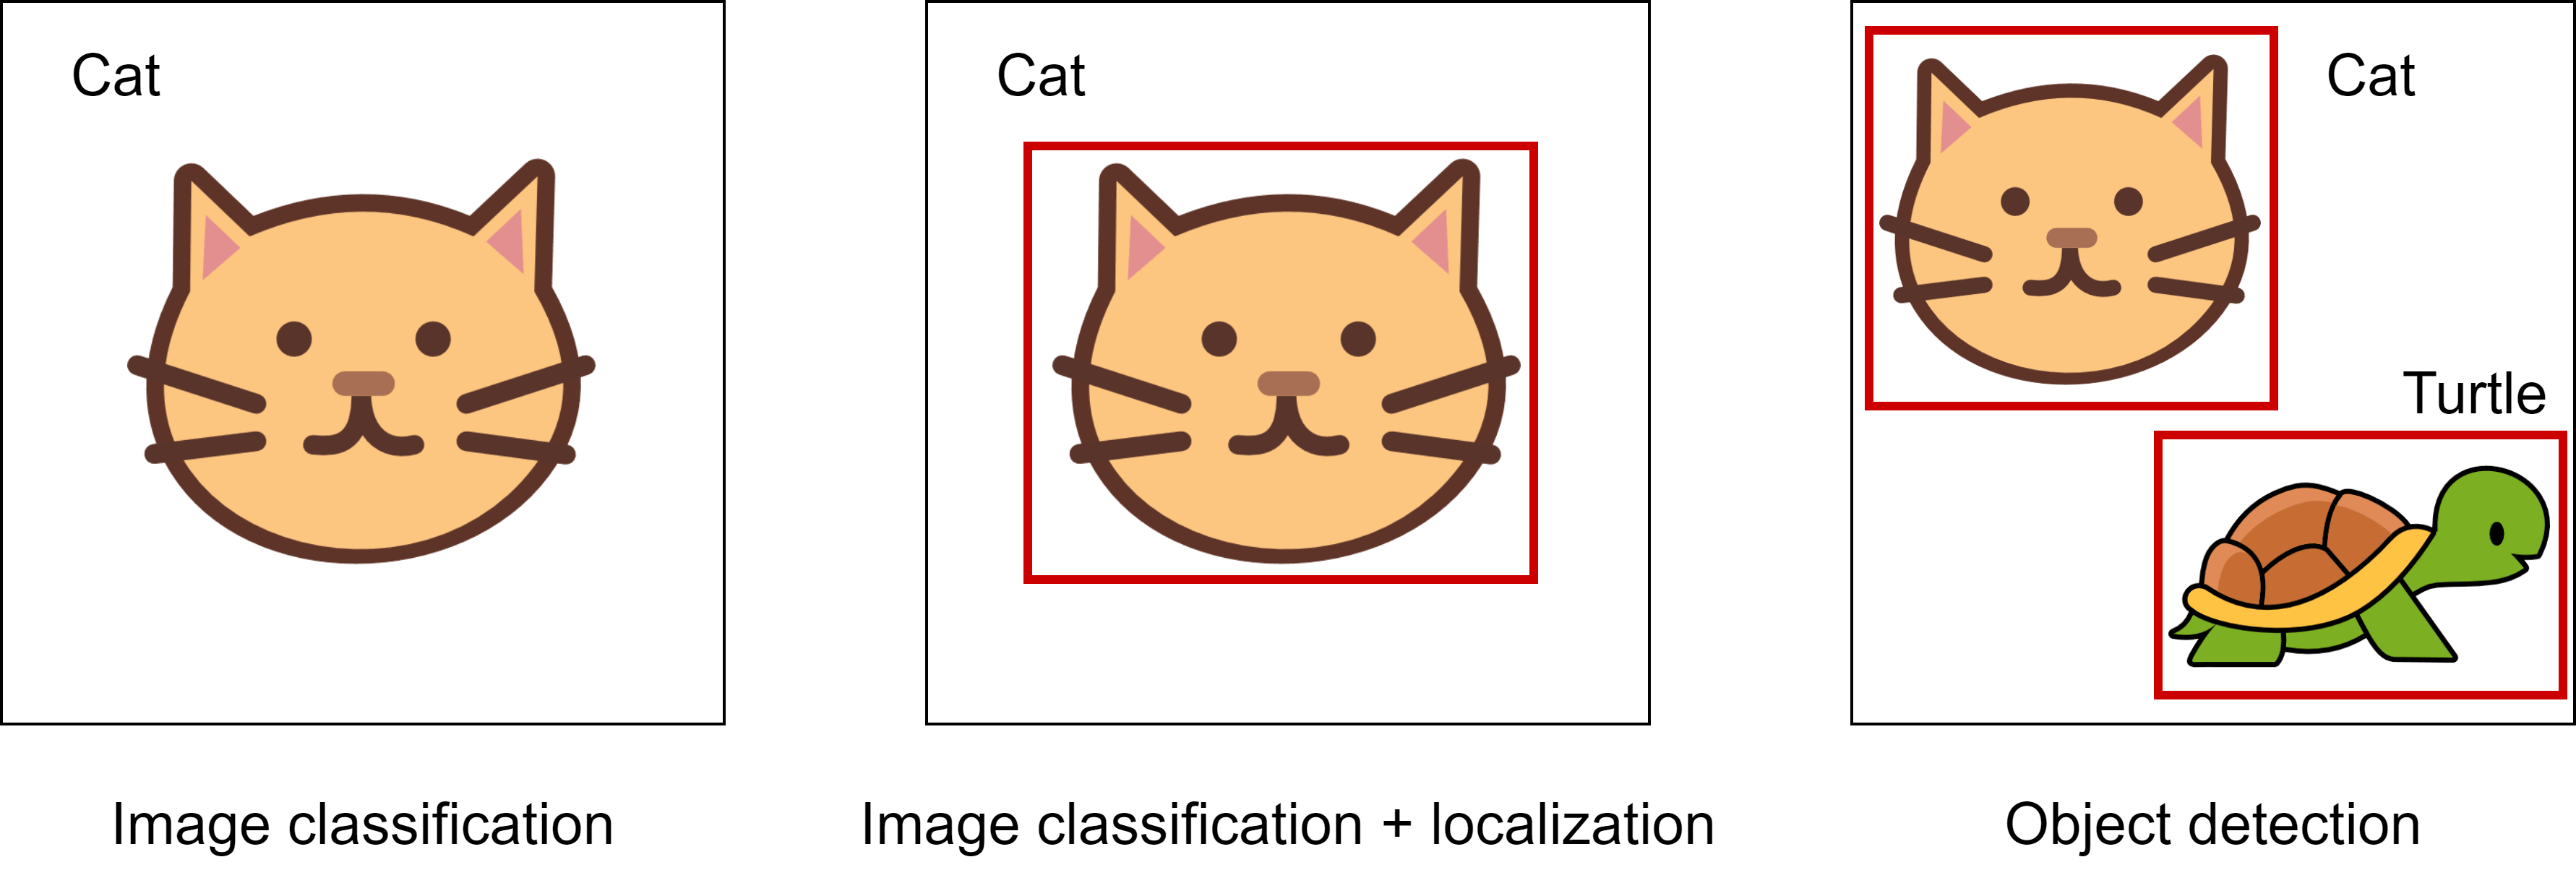
\includegraphics[width = 1\textwidth]{image/Image classification & Object detection.png}
        \caption{Difference between image classification, image localization and object detection}
        \label{fig: IC&OD}
    \end{figure*}

    In image classification, the most common types are binary classification \cite{zhuang2019structured}, multiclass classification \cite{murthy2016deep} and multilabel classification \cite{tsoumakas2008multi}. As the name implies, in binary classification, there are only two possible outcomes when identifying an image. For instance, if the model's labels are cat and dog, the prediction can only be either a cat or a dog. Conversely, multiclass classification means that the image can belong to multiple possible classes instead of two classes. Using the previous example, the prediction in multiclass classification could be a cat, dog, elephant, snake, or other different animals, rather than choosing between just two labels. It is important to note that the final prediction in both binary and multiclass classification will result in only one label. If an image needs to have multiple labels, a different type of image classification model is required, such as a multilabel model.

    The process of training an image classification model is generally similar to what is described in section 2.2.1 on Deep Learning. In image classification, commonly used datasets include: ImageNet \cite{5206848}, CIFAR-10, CIFAR-100, and MNIST \cite{deng2012mnist}. It's worth mentioning that we often perform preprocessing on images. Common preprocessing techniques include image cropping, image resizing, and image normalization. Image cropping is a technique that removes the unnecessary parts of the image. Through image cropping, the irrelevant parts of the image will be removed. As shown in the figure \ref{fig: imageCropping}, the pink area in the original picture is removed to prevent model from learning the useless information. Image resizing ensures that all images are of the same size, which helps improve computational speed. However, there is a potential risk of degrading the model's performance by using image resizing \cite{relationshipBetweenImageSizeAndQuality}. Hence, the size of the resized images is typically determined based on actual requirements. Normalizing images also helps the model learn from each image more effectively. After preprocessing, we usually use pretrained models instead of designing a new model architecture from scratch. This approach enhances computational efficiency and results. Common image classification models used include InceptionV3 \cite{szegedy2015rethinkinginceptionarchitecturecomputer}, ResNet \cite{he2015deepresiduallearningimage}, and others.
    \begin{figure*}[htbp]
        \centering
        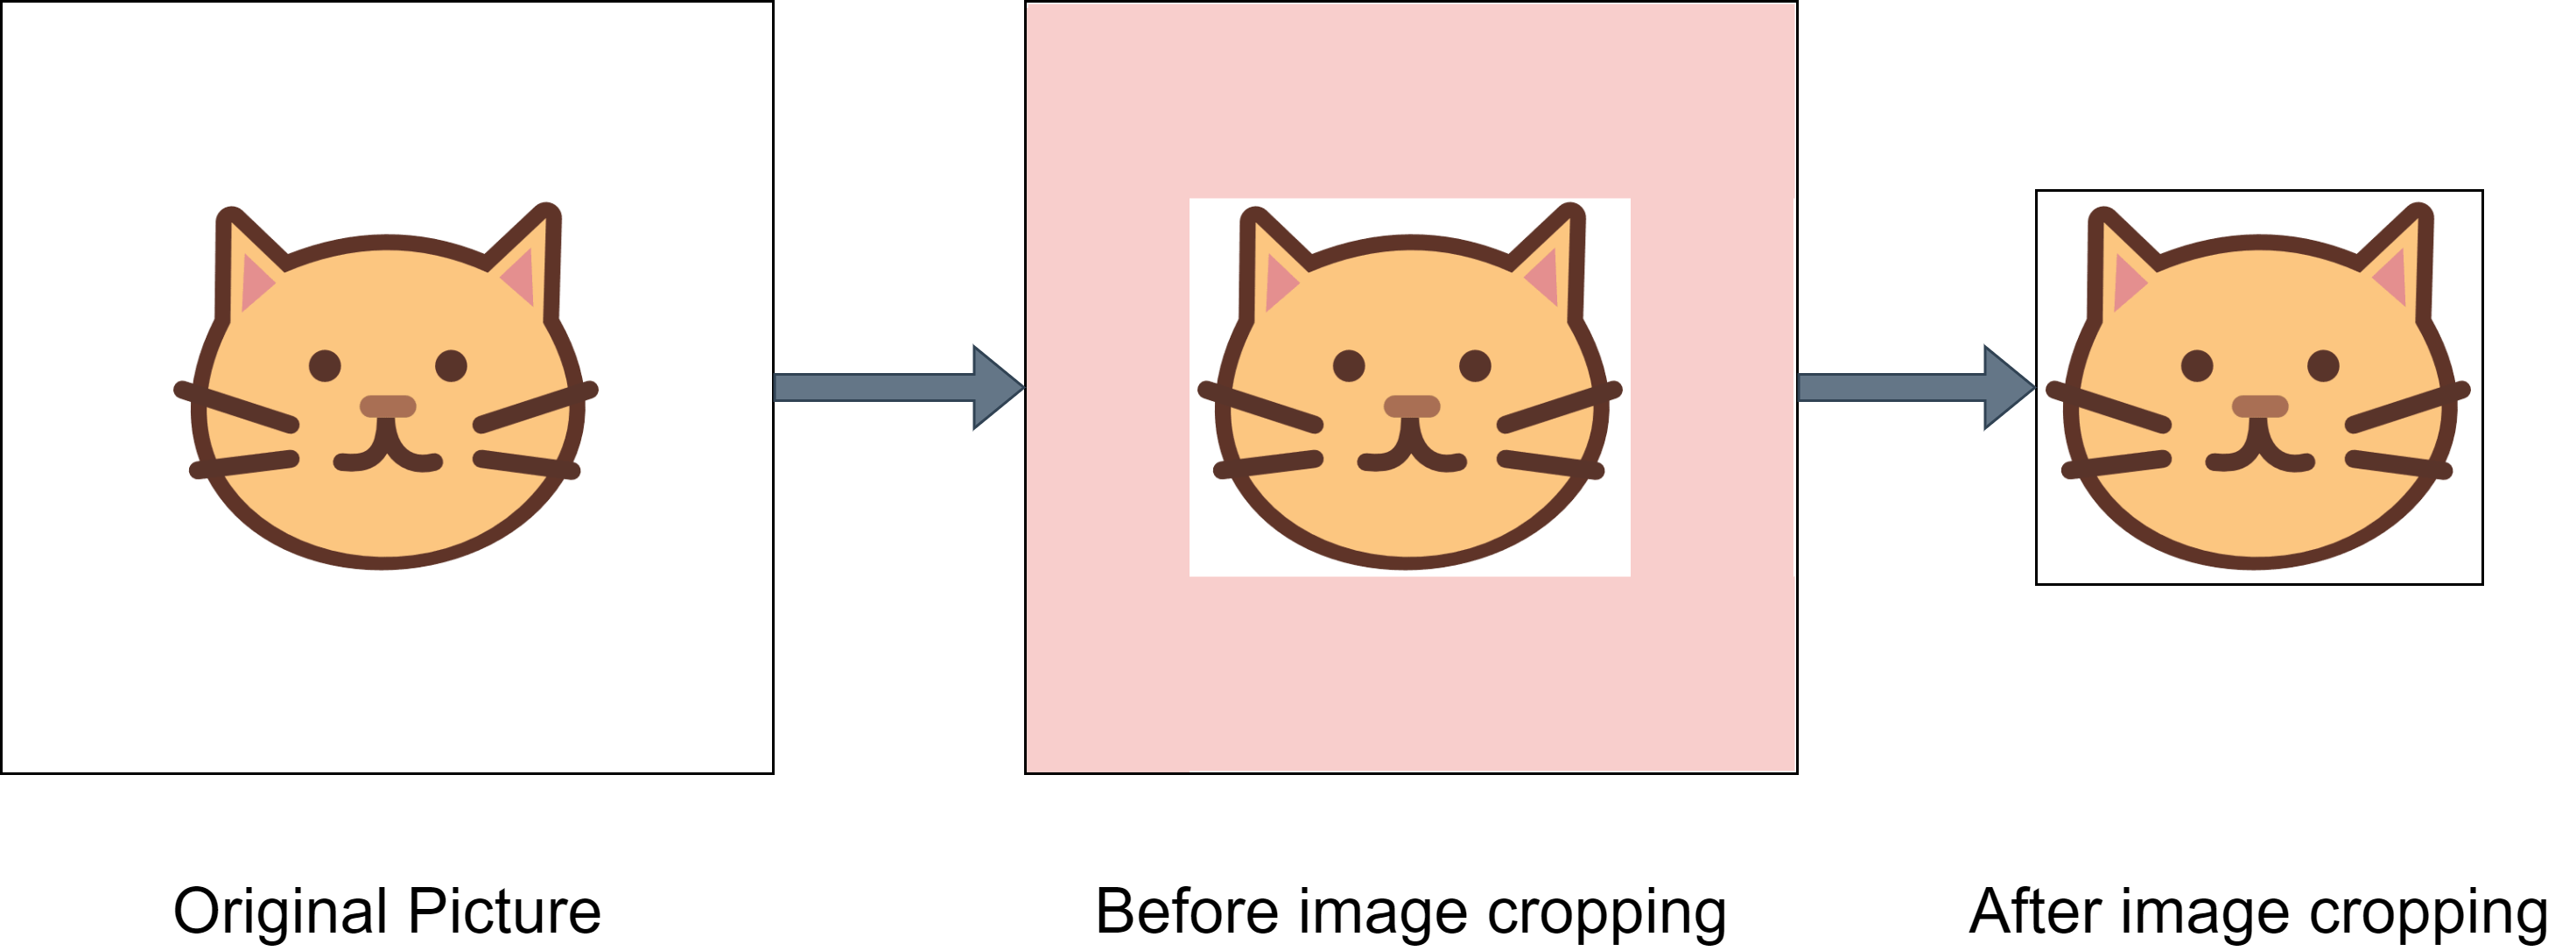
\includegraphics[width = 1\textwidth]{image/ImageCropping.png}
        \caption{The process of image cropping}
        \label{fig: imageCropping}
    \end{figure*}

    In the real world, image classification can be applied in many areas. For example, it can be used in medical imaging to identify tumors in X-rays. It can also be employed in autonomous vehicles to quickly recognize objects surrounding the vehicle. Facial recognition is another application of image classification, used for company access control and as a method to unlock personal devices such as phones or computers.
    % \subsection{}
    % 定義定義定義定義定義定義\cite{latex2e},定義定義定義定義,定義定義定義定義定義定義定義定義定義定義,定義定義。

    % \begin{table*}[htbp]
    %     \centering
    %     \caption{表格範例標題} \label{tab: complexity}
    %     \makebox[\linewidth][c]{
    %     \renewcommand\arraystretch{1.2}{
    %         \begin{tabular}{| l | c  c  c  c |}
    %         \hline
    %         Protocol & $P$ & $CS_1$ & $CS_2$ & $RG$ \\
    %         \hline
    %         MSSMul & $O(1)$, $O(1)$, N/A & $O(n-t)$, $O(n)$, $O(1)$ & $O(n-t)$, $O(n)$, N/A & $O(1)$, $O(n)$, $O(n)$ \\
    %         SC & $O(1)$, $O(1)$, N/A & $O(n-t)$, $O(n)$, $O(1)$ & $O(n-t)$, $O(n)$, N/A & $O(1)$, $O(n)$, $O(n)$ \\
    %         \hline 
    %         \end {tabular}
    %     }}
    % \end {table*}

    % \section{模型說明(小標)}

    % 說明說明說明說明,說明說明說明說明說明說明說明說明說明說明說明說明,說明說明說明說明說明說明說明說明。

    % \begin{figure*}[htbp]
    %     \centering
    %     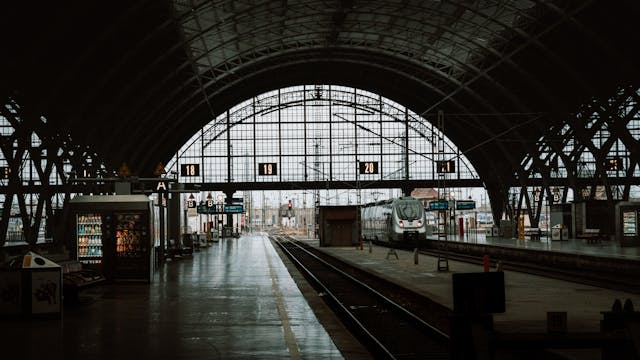
\includegraphics[width = 0.5\textwidth]{image.jpeg}
    %     \caption{Cool train station}
    %     \label{fig: image}
    % \end{figure*}

\end{ZhChapter}